\chapter{Analisi del sistema}

\section{Introduzione}

\section{Diagrammi di attività}
\begin{center}
	\begin{tabularx}{\textwidth}{ l X } 
		\toprule
			\formattaTitoloTab{ID} & \formattaTitoloTab{Caso d'uso di riferimento} \\
		\cmidrule(l{\cmidrulekern}r{\cmidrulekern}){1-2}
		\newAttivita{da:login}{\formattaAT}{Login} & \getIDTitletodesc{cu:login} \\ 
		\addlinespace[1em] 
		\newAttivita{da:logout}{\formattaAT}{Logout} & \getIDTitletodesc{cu:login} \\ 
		\addlinespace[1em] 
		\newAttivita{da:iscrizione}{\formattaAT}{Iscrizione} & \getIDTitletodesc{cu:login} \\ 
		\addlinespace[1em] 
		\newAttivita{da:approvazione}{\formattaAT}{Approvazione iscrizione} & \getIDTitletodesc{cu:login} \\ 
		\addlinespace[1em]
		\newAttivita{da:schedaprodotto}{\formattaAT}{Inserimento prodotto} & \getIDTitletodesc{cu:login} \\ 
		\bottomrule
	\end{tabularx}
\end{center}
\subsectionDA{da:login}
\begin{center}
			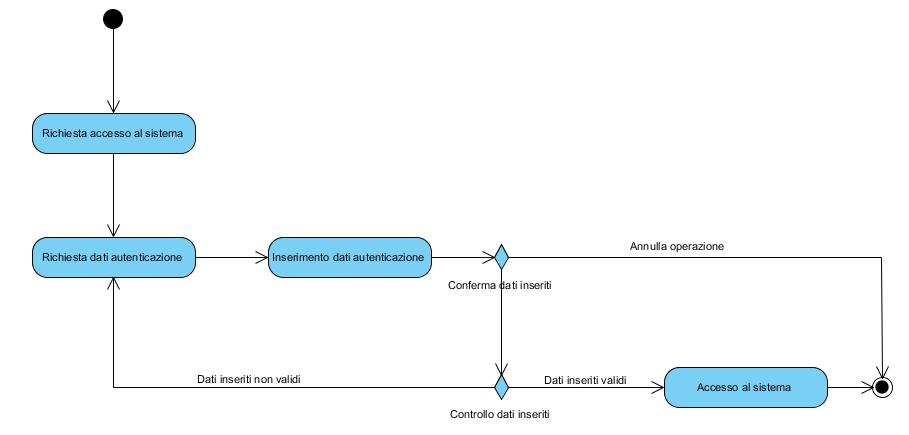
\includegraphics[width=\textwidth]{assets/visualParadigm/attivita/login}
\end{center}

\subsectionDA{da:logout}
\begin{center}
	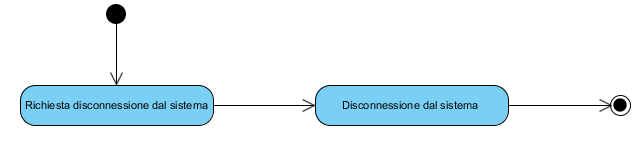
\includegraphics[width=\textwidth]{assets/visualParadigm/attivita/logout}
\end{center}

\subsectionDA{da:iscrizione}
\begin{center}
	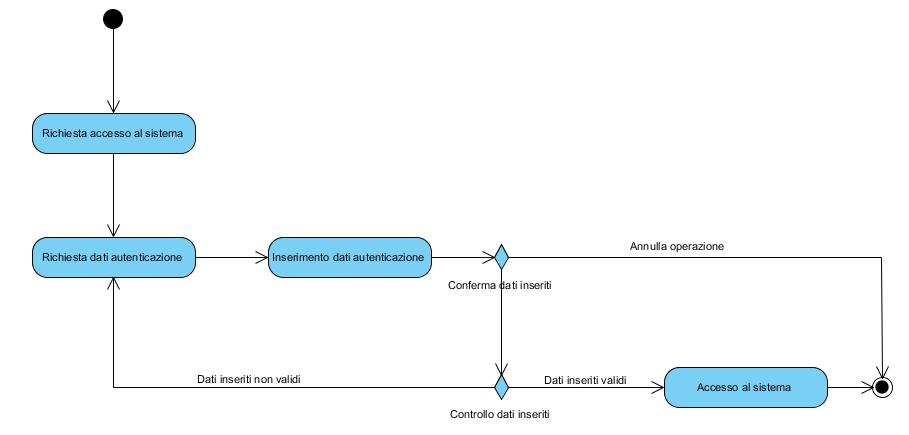
\includegraphics[width=\textwidth]{assets/visualParadigm/attivita/login}
\end{center}

\subsectionDA{da:approvazione}
\begin{center}
%	\includegraphics[width=\textwidth]{assets/visualParadigm/attivita/approvazioneiscrizione}
\end{center}

\subsectionDA{da:schedaprodotto}
\begin{center}
	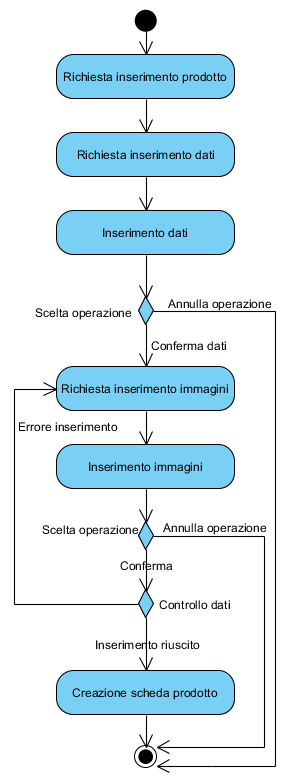
\includegraphics[width=\textwidth]{assets/visualParadigm/attivita/schedaprodotto}
\end{center}

\begin{comment}
	CU.A.1 - Login
	CU.A.3 - Logout
	CU.B.1 - Iscrizione tramite modulo
	CU.B.2 - Iscrizione tramite Social Network
	CU.B.3 - Iscrizione tramite approvazione
	CU.B.4 - Approvazione iscrizione
	CU.C.5 - Inserimento scheda prodotto
	CU.G.1 - Inserimento valutazione
	CU.H.1 - Inserimento recensione
	CU.H.4 - Commento a recensione
	CU.H.5 - Giudizio recensione
	CU.I.1 - Follow account
	CU.I.2 - Unfollow account
	CU.K.1 - Ricerca prodotto
	CU.K.2 - Ricerca profilo
	CU.K.3 - Ricerca notizia
	CU.M.1 - Mostra vetrina
	CU.M.2 - Mostra scheda prodotto
	CU.M.3 - Mostra recensioni associate al prodotto
	CU.M.4 - Mostra recensione
	CU.M.5 - Mostra profilo pubblico
	CU.M.6 - Mostra notizia
	CU.M.7 - Mostra aggiornamenti dai followed
\end{comment}
